\documentclass{atlasnote} 

%\documentclass[usetikz]{atlasnote} % the 'usetikz' option loads tikz.sty in the proper place, 
                                   % avoiding conflicts with graphicx.sty.
                                   % Don't know what tikz.st is? Just ignore this line! :-)

%\documentclass[coverpage]{atlasnote} % the 'coverpage' option loads the ATLAS Cover Page package 
                                      % ans makes sure that the cover page is generated before the
                                      % note title page. Make sure that the latest version of
                                      % of 'atlascover.sty. is installed on your system!

%\usepackage{graphicx} % This is already loaded by the atlasnote class
                       % Just use it to include your plots!

%\usepackage{atlasphysics} % Contains useful shortcuts. Uncomment to use
                           % See instruction.pdf for details

%%%%%%%%%%%%%%%%%%%%%%%%%%%%%%%%%%%%
%           Title page             % 
%%%%%%%%%%%%%%%%%%%%%%%%%%%%%%%%%%%%

\skipbeforetitle{100pt}

% Title
\title{Monitoring of computing resource utilization of the ATLAS experiment}

% if multiple authors/affiliations are needed, use the authblk package
\usepackage{authblk}
\renewcommand\Authands{, } % avoid ``. and'' for last author
\renewcommand\Affilfont{\itshape\small} % affiliation formatting

\author[a]{David Rousseau}
\author[b]{Gancho Dimitrov}
\author[a]{Ilija Vukotic}
\author[c]{Osman Aidel}
\author[a]{RD Schaffer}
\author[d]{Solveig Albrand}

\affil[a]{LAL, Univ. Paris-Sud and CNRS/IN2P3, Orsay, France}
\affil[b]{CERN, Geneva, Switzerland}
\affil[c]{Domaine scientifique de la Doua, Centre de Calcul CNRS/IN2P3, Villeurbanne Cedex, France}
\affil[d]{Laboratoire de Physique Subatomique et de Cosmologie, Universit ́e Joseph Fourier and CNRS/IN2P3 and Institut National Polytechnique de Grenoble}

% Date: if not given, uses current date
%\date{\today}

% Draft version: if given, adds draft version on front page, a
% 'DRAFT' box on top of each other page, and line numbers to easy
% commenting. Comment or remove in final version.
\draftversion{1.0}

% Journal: adds a 
% \journal{Phys. Lett. B} 

% Abstract
\abstracttext{
  Due to the good performance of the LHC accelerator, the ATLAS experiment has seen higher than anticipated levels for both the event rate and the average number of interactions per bunch crossing. In order to respond to these changing requirements, the current and future usage of CPU, memory and disk resources has to be monitored, understood and acted upon. This requires data collection at a fairly fine level of granularity: the performance of each object written and each algorithm run, as well as a dozen per-job variables, are gathered for the different processing steps of Monte Carlo generation and simulation and the reconstruction of both data and Monte Carlo. We present a system to collect and visualize the data from both the online Tier-0 system and distributed grid production jobs. Around 40 GB of performance data are expected from up to 200k jobs per day, thus making performance optimization of the underlying Oracle database of utmost importance.
}

%%%%%%%%%%%%%%%%%%%%%%%%%%%%%%%%%%%%
%            Content               % 
%%%%%%%%%%%%%%%%%%%%%%%%%%%%%%%%%%%%

\begin{document}

% Test of tikz.sty loadin in atlasnote.cls. Use 'usetkiz' option in documentclass declaration:
% e.g. \documentclass[usetikz]{atlasnote}
% \input{tikz-test}

\section{Introduction}


The main goal of this system is to provide the following information:
\begin{itemize}
	\item size of all the objects that ATLAS stores in all officially produced data files.
	\item timing of all the algorithms, tools and services used during official data production, simulation, and reconstruction.
	\item CPU time, wall clock time, memory leakage and other per job information 
\end{itemize}

This information will be used:
\begin{itemize}
	\item by performance experts to identify places where optimization will be most beneficial
	\item by management to determine current resource needs and to extrapolate for future running parameters
	\item by reco shifters to continuously monitor changes in resource consumption
	\item example1: find all the persistent objects not written out in last 1 year and remove them from the code.
	\item example2: find all the unneeded persistent objects written out.
	\item example3: find all the algorithms, tools or services not needed in a particular transformation step.
	\item example4: estimate resources needed for a particular MC/real data production/reconstruction. 
\end{itemize}


In this document we will use term {\bf "task"} to signify operation (eg. reconstruction) on the data set containing one or more files and {\bf "job"} to signify part of the task usually executed on one core and one input file. While jobs can are usually very complex and involve multiple execution steps they are atomic operations ie. we consider job as failed in case of error in any part of it and all of its results are discarded.

The production system is schematically presented in Figure~\ref{fig:sysschema}. It is composed of two main parts: the Tier-0 and the grid.

The Tier-0 having around 6000 processing cores is tasked with the initial real data reconstruction. It also reconstructs all the special streams: calibration, debug, express etc. As a calibration loop has to be finished inside 36 hours long delays are no allowed. Since the jobs take roughly 10 hours even one failed job can introduce serious delays. For this reason failing a job due to resource monitoring is not an option, any problem in monitoring is just reported and the transform continues.

The grid production system can be used for both reconstruction of real data and all the steps of MC production. The system is capable of running 200 thousand jobs per day. While requirements on delays are not as strict as at Tier-0, job failing due to monitoring is also not acceptable since even very small percentage of fail jobs would mean a significant overhead for the production shifters.  

\begin{figure}
  \centering
  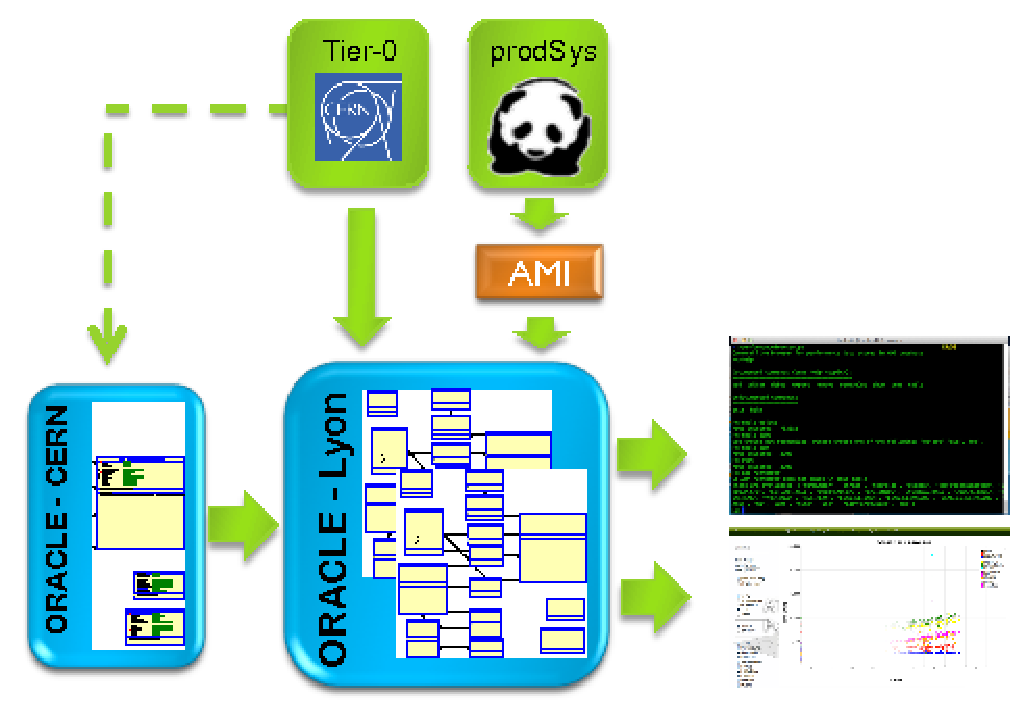
\includegraphics[width=\columnwidth]{sysschema}
  \caption{Organization of the Atlas resources usage monitoring system.}
  \label{fig:sysschema}
\end{figure}

Allowing monitoring to quietly fail can lead to not having resource usage information from all of the events. It can also happen that a job fails after it already sent part of the information to the DB. The job is then restarted and this leads to these events having twice the statistical weight. Both of these effects should not matter for most of applications. In case of MC collecting information from even small percentage of jobs is sufficient. We assume that sampling just 20\% of all the jobs will give us good enough cross-section of hardware and middleware resources used.  For the real data majority of jobs is good enough. While resources are uniformed, time dependent changes in for example trigger settings, average number of interactions per bunch crossing, etc can make big difference in amount of resources used.
    
All of the monitoring system is composed of 4 functional parts: information collection, data transport, data storage, and visualization. We will briefly describe each.

\section{Data collection}
The first problem we had to solve is how to distinguish production jobs. 
All of the production jobs are actually executions of the same script (Reco_trf.py) with different parameters. The parameters define input and output files, calibration constants etc. The Reco transform executes an appropriate sequence of Athena sub-jobs.  
While this can be changed for now we settled at:

    stored object size is obtained from PoolFile.py root based tool (also used by checkFile.py) that opens root file and returns names, sizes and number of entries of all the collections stored.
    algorithm timings are currently obtained from PerfMonSD. (Data collected before 1st April were obtained through ChronoSvc).
    per job information is obtained from PerfMonSD. This in turn obtains this information from operating system. 

Code collecting the information is situated in the doPostRunActions function of the Tools/PyJobTransformsCore/trf.py.

\section{Data transport}

    Tier-0 collected data are sent directly to Oracle DB in Lyon. Authentication is done via environment variable TZAMIPW. In case that the default db is unreachable Oracle DB in CERN is used to temporarily store the data, from where data are moved automatically to Lyon.
    prodSys (grid) jobs data are sent using special AMI commands. Authentication is done via VOMS. Only jobs having '/atlas/Role=production' in output of voms-proxy-info -fqan will try to send data. 

Currently there is no backup solution in case of problems with AMI. In both cases it is guaranteed that if upload fails for whatever reason it will fail quietly and jobs will finish normally. There is a window of 60 seconds in which all of the data collection and delivery has to be done. All the code concerning data transport is in Tools/PyJobTransforms.

\section{Data storage}
Database scheme may be found here. For now there is no documentation describing all the stored procedures that are running on the db and which summarize the data received. In order to ease certain common tasks a table with run info is included in the data base. It contains:

    mu - average mu - from the plots like these
    lumi - luminosity
    time - duration of the run
    use - flag saying if this run is ok to use. It is manually set. It can be used to exclude runs where information is messed up.
    ReadyForPhysics - flag obtained from AMI db. All the runs having this flag set to True are distributed. 

This table is updated by the script perfStatusOfAmi.py run by cron job every day at 13:00.


\section{Data mining}
How to use it?
Classify objects/algorithms
Independently what type of visualization you will use, and unless you are interested in only job performance data, you should always first make sure objects/algorithms are all properly classified. This is done through AMI interface. Path to it:

    Start from the AMI home page (AMI home).
    In the menu find: Applications->Atlas->AMI admin
    Now menu has changed and you have in it also Database option
    Click on it and you have a large list of the databases. You need the one named: \begin{verbatim}COLL_SIZES_01\end{verbatim}
    Click on it (not on "+" sign) and than bookmark this page as you'll need it. This bookmark is not the one from your browser but the one from AMI (you'll see it in the menu)
    Now click on \begin{verbatim}ATLAS_AMI_COLL_SIZES_01_LAL\end{verbatim} in 'database name' will give you list of all the relevant tables. For the details on the table schema click on table name. To look at the data in the table click on the link (Browse). For the classification purposes two table are important ones AlgoRef and object. 

Initial object classification was done by hand. Objects are separately classified for all the data formats (AOD,ESD,DPD,...) Algorithms are classified by a script Tools/PerformanceReports/updateAlgoCategories.py. The script is kept up to date by ThomasKittelmann. Currently the only persons having necessary rights to make changes in classification are DavidRousseau, IlijaVukotic, ThomasKittelmann and RD Schaffer.

NEVER CHANGE INFO IN OTHER TABLES UNLESS YOU KNOW EXACTLY WHAT ARE YOU DOING - for example removing category or stream name will delete all the data ever classified in this category/stream.

Place your content here. Policy~\cite{publication_policy}

Place your content here Appendix~\ref{app:DBaccounts}

Place your content here Appendix~\ref{app:DBschema}

Place your content here Appendix~\ref{app:DBopt}

\section{Performance}
here on what percentage of info was collected.
what is time to upload
what is cpu load produced

\section{Conclusion}
Do we find this system to work ok for this kind of task and this data size. How much it could expand.

%%%%%%%%%%%%%%%%%%%%%%%%%%%%%%%%%%%%%%%%%%%%%%%%%%%%%%%%%%%%%%%%%%%%%%%%%%%%%%%
% Bibliography
%%%%%%%%%%%%%%%%%%%%%%%%%%%%%%%%%%%%%%%%%%%%%%%%%%%%%%%%%%%%%%%%%%%%%%%%%%%%%%

\bibliographystyle{atlasnote}
\bibliography{performance_monitor_note}


%%%%%%%%%%%%%%%%%%%%%%%%%%%%%%%%%%%%%%%%%%%%%%%%%%%%%%%%%%%%%%%%%%%%%%%%%%%%%%%
% Technical Aspects
%%%%%%%%%%%%%%%%%%%%%%%%%%%%%%%%%%%%%%%%%%%%%%%%%%%%%%%%%%%%%%%%%%%%%%%%%%%%%%%

\newpage
\appendix
\part*{Appendices}
\addcontentsline{toc}{part}{Appendices}

\section{Database accounts} \label{app:DBaccounts}
accounts are : ...
servers are: ...
which ones are used: ...
\section{Database schema} \label{app:DBschema}
schema looks like this: figure

\section{Database optimization} \label{app:DBopt}
all of the partitionings, row movements, re-indexings

\end{document}